\selectlanguage{french}
\Chapter{OBJECTIFS DE LA RECHERCHE}\label{sec:Objectifs}

\section{Analyse des lacunes dans les connaissances actuelles}

Le procédé de soudure par résistance des composites thermoplastiques avec un élément chauffant en acier inoxydable est un procédé simple qui offre de bonnes propriétés mécaniques et qui peut facilement être mis à l'échelle. 
Sa faiblesse réside dans le manque d'interactions entre le polymère et l'élément chauffant. 
Celle-ci peut être contournée de deux façons: \begin{inparaenum}[a)]
	\item en effectuant des traitements de surface permettant d'augmenter l'adhésion entre la matrice et l'acier inoxydable ou 
	\item en changeant la nature de l'élément chauffant. 
\end{inparaenum}
En ce qui concerne la première solution, des travaux de recherche sont en cours à l'École de technologie supérieure afin d'explorer cette option. 
Pour la seconde solution, un élément chauffant constitué d'un nanocomposite conducteur sera employé. 
Le polymère de la matrice de ce nanocomposite devra pouvoir diffuser au travers du polymère des adhérents et l'ajout de particules conductrices le rendra conducteur. 
Ainsi, le nanocomposite développé servira à la fois d'élément chauffant et offrira une zone riche en polymère pour produire une soudure. 
Bien entendu, la conductivité électrique du nanocomposite ne pourra certainement pas atteindre celle de l'élément chauffant en acier inoxydable. 
Sa plus faible conductivité fera en sorte que le nanocomposite aura une résistance électrique beaucoup plus élevée. 
Il sera alors possible de tirer parti de cette résistance pour utiliser le nanocomposite comme élément chauffant. 
Cette solution est inexplorée dans les articles précédemment publiés. 

La possibilité de souder un élastomère thermoplastique avec un autre polymère rigide reste également inexplorée dans les écrits recensés. 
Dans le meilleur des cas, un mélange biphasique avec un élastomère et un autre polymère est utilisé dans une jonction, mais sans obtenir de diffusion entre les phases \cite{Hollande1998}. 
Aucun cas documenté de soudage mixte entre un élastomère et un autre polymère n'a été trouvé. 

Ainsi, nous pouvons définir deux besoins de recherche: d'abord en ce qui concerne la production d'un élément chauffant nanocomposite permettant la soudure par résistance de composites thermoplastiques, ensuite en ce qui a trait à l'obtention d'une soudure mixte avec un élastomère. 

\section{Objectifs}
\label{sec:objectifs}

En considérant l'ensemble des connaissances publiées et des besoins du partenaire industriel, voici la liste des objectifs sur lesquels se concentreront ces travaux. 

\begin{enumerate}
	\item Concevoir un élément chauffant nanocomposite conducteur en tenant compte des propriétés électriques et thermiques nécessaires au procédé de soudage par résistance. 
	\item Développer un procédé de soudage par résistance avec un élément chauffant nanocomposite entre deux adhérents en composite à matrice thermoplastique. 
	\item Établir une fenêtre d'opération pour le soudage par résistance avec un élément chauffant nanocomposite entre deux adhérents en composite à matrice thermoplastique. 
	\item Développer un procédé de soudage par résistance avec un élément chauffant nanocomposite entre un adhérent en composite à matrice thermoplastique et un adhérent en élastomère thermoplastique. 
\end{enumerate}

\section{Cibles de performance}

Afin d'évaluer l'atteinte des objectifs et pour aider à la sélection des matériaux, ArianeGroup a fourni des cibles de performance calquées sur les caractéristiques de la solution actuelle pour les composites à matrice thermodurcissable. 
Voici deux des principaux requis techniques concernant la jonction soudée. 

\begin{enumerate}
	\item Résistance en cisaillement supérieure à \SI[locale=FR]{14}{\mega\pascal}. 
	\item Rupture cohésive de l'élastomère. 
\end{enumerate}

\section{Éléments méthodologiques}

Avant de procéder au développement d'un élément chauffant nanocomposite, des essais préliminaires ont permis d'établir certains paramètres expérimentaux. 

\subsection{Choix du polymère pour la matrice de l'élément chauffant nanocomposite}

Pour la matrice du nanocomposite, des essais initiaux ont démontré la possibilité d'employer du PEEK. 
Cependant, tôt dans la conception du projet, il a été remarqué que la résistance thermique de l'élastomère serait le facteur limitant du procédé de soudage multimatériaux. 
Afin de limiter la température du procédé de soudage, il a été décidé d'employer une matrice de PEI en raison de sa miscibilité avec le PEEK \cite{Torre1992,Crevecoeur1991}. 
De plus, en raison de l'impact de la masse moléculaire sur le temps de reptation des chaines, il a été décidé d'employer un PEI à faible masse moléculaire pour maximiser les chances d'obtenir des jonctions soudées. 
Cette décision aura cependant un impact sur les résistances mécaniques obtenues lors des essais de caractérisation. 

\subsection{Conception de l'élément chauffant nanocomposite}

Après avoir déterminé le polymère composant la matrice du nanocomposite, une cible de conductivité électrique a été établie. 
Cette cible a été définie de façon à limiter le voltage appliqué durant le procédé de soudage tout en considérant la puissance thermique devant être dégagée durant le procédé. 
L'équation \ref{EQ:conductivite} permet d'évaluer la conductivité électrique nécessaire ($\sigma$) pour dégager une puissance ($P$) définie en fonction de la géométrie du conducteur ($l$ et $A_s$) et de la tension électrique ($V$). 

\begin{equation}
\label{EQ:conductivite}
\sigma = \frac{P \times \frac{l}{A_s}}{V^2}
\end{equation} 

En tenant compte des dimensions prévues de l'élément chauffant et pour une puissance surfacique de \SI[locale=FR]{350}{\kilo\watt\per\square\metre}, une application directe de cette formule permet de calculer qu'une conductivité électrique entre 45 et \SI[locale=FR]{1,8e4}{\siemens\per\metre} est nécessaire afin de maintenir un voltage dans une plage entre 5 et \SI[locale=FR]{100}{\volt}. 
En raison des faibles conductivités électriques pouvant être obtenues pour des nanocomposites conducteurs, il a seulement été possible de développer des nanocomposites conducteurs avec une conductivité électrique s'approchant de la limite inférieure. 
Il a été décidé de viser une cible de conductivité électrique de \SI[locale=FR]{100}{\siemens\per\metre} pour l'élément chauffant nanocomposite. 
Cette cible se situe près des limites supérieures des mesures de conductivité électrique rapportées dans la littérature et est généralement peu explorée. 
Ce choix a un impact sur le voltage nécessaire lors du soudage.
Une attention particulière a donc été portée afin de limiter les fuites de courant dans les adhérents. 

\subsection{Choix des charges conductrices}

Sur le plan de la morphologie, le PEI du nanocomposite sert à tenir en place un réseau de charges conductrices qui à leur tour permettent d'atteindre la cible de conductivité nécessaire au procédé de soudage. 
Cette conception d'un élément chauffant n'est pas très éloignée de la conception conventionnelle qui emploie un grillage en acier inoxydable entre deux films de polymères. 
Dans ces deux cas, la matrice est présente pour fournir une zone riche en résine pour favoriser le soudage. 

Afin d'atteindre la cible de conductivité électrique établie, plusieurs compositions de nanocomposites ont été évaluées. 
Tout d'abord, une évaluation des couts a permis de déterminer que des nanocomposites conducteurs de PEI avec des nanofils d'argent auraient un cout de revient de l'ordre de 30 à 70\$ par gramme contre un cout d'environ 0,40\$ par gramme pour les nanocomposites avec des nanotubes de carbone à haute pureté. 
En raison de l'échelle visée pour le procédé de soudage, les nanofibres d'argent ont été mises de côté vu leur cout trop élevé. 
Pour les nanofibres de cuivre, leur cout évalué entre 0,90 et 1,30\$ par gramme les rendait également plus couteux que les charges à base de carbone. 

Les charges conductrices évaluées lors des essais initiaux étaient des nanotubes de carbone multiparois avec une pureté de 99\% et de 95\% (produits par Raymor Industries), des nanofibres de carbone (grade PR--19--XT--LHT produites par Pyrograf Products inc.) ainsi que des nanoplaquettes de graphène (xGnP grade C-300 produites par XGSciences). 
Ces charges ont été mélangées à du PEI avec des fractions massiques allant jusqu'à 15\%.
La conductivité électrique des mélanges obtenus par extrusion a été évaluée à l'aide d'un système de mesure à 4 pointes. 
La figure \ref{fig:conductivite_lin} présente les résultats des mesures de conductivité électrique. 

\begin{figure}[h]
	\centering
	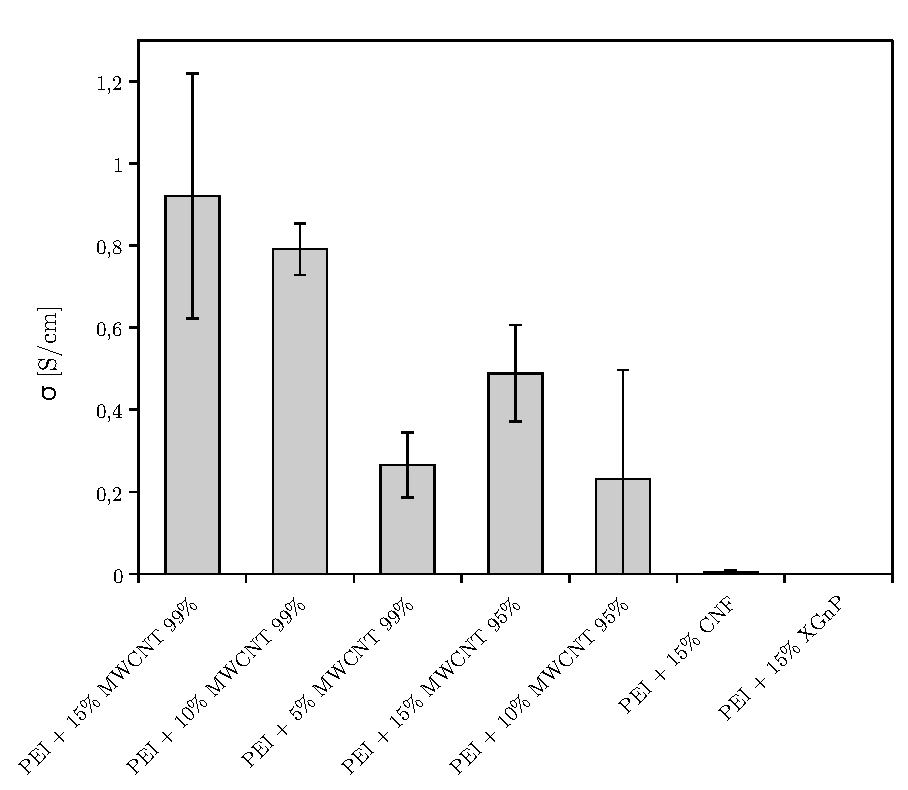
\includegraphics[width=0.75\textwidth]{conductivity_lin.pdf}
	\caption{Conductivité de mélanges de PEI et de particules conductrices}
	\label{fig:conductivite_lin}
\end{figure}

La composition retenue pour le projet est un nanocomposite de PEI avec 10\% massique de nanotubes de carbone avec une pureté de 99\%. 
La fraction de nanotubes employée dépasse de beaucoup la fraction nécessaire pour atteindre le seuil de percolation.
Le nanocomposite obtenu se trouve dans la portion presque linéaire de la courbe de conductivité électrique où l'ajout d'une grande quantité de charges est nécessaire pour obtenir une augmentation modeste de la conductivité électrique (Fig. \ref{fig:percolation_electrique}). 
Les variations de la conductivité électrique causées par le contrôle de la composition du nanocomposite sont moins prononcées dans cette portion de la courbe, puisque cette région ressemble à un plateau avec une faible pente contrairement à la variation brusque à proximité du seuil de percolation. 
L'emploi d'un nanocomposite avec une telle composition a pour but de préserver la conductivité électrique à l'état fondu en maximisant les possibilités de maintenir le réseau électrique percolé. 

L'option d'employer un nanocomposite de PEI avec 15\% massique de nanotubes de carbone avec une pureté de 99\% a été considérée, mais rejetée en raison de la grande variabilité entre les mesures de conductivité. 
La variabilité observée peut s'expliquer par un plus grand niveau d'agglomération des nanotubes.  
Le mélange par extrusion, avec les paramètres employés, ne permettait pas de désagglomérer les nanotubes aussi efficacement qu'avec un mélange à 10\% massique. 
Également, les nanocomposites obtenus avec 15\% massique de nanotubes de carbone étaient beaucoup plus cassants en raison d'une grande réduction de leur ductilité. 
Un dernier élément ayant mené au rejet du mélange à 15\% massique est le modeste gain en conductivité électrique obtenu malgré une augmentation de 50\% de la quantité de nanotubes et du cout associé. 

\subsection{Méthode d'évaluation de la dispersion des charges}

Comme discuté au chapitre \ref{sec:RevLitt}, pour tirer profit des propriétés de conductivité électrique des nanoparticules, il est important de bien disperser les nanocharges tout en maintenant un certain niveau de contact. 
L'évaluation de l'état de dispersion peut être réalisée entre autres au microscope électronique à balayage ou avec un microscope à force atomique. 
Les images obtenues peuvent ensuite être analysées pour évaluer la dispersion. 
Des techniques existent même pour quantifier objectivement l'état de dispersion de particules \cite{Bray2011,Bray2012}. 
Le facteur de forme ou la morphologie des charges évaluées doivent également être considérés dans cette analyse \cite{Bray2013a,Sul2011}. 

L'imagerie au microscope électronique à balayage a déjà été appliquée à l'analyse de dispersion de petites quantités de nanoparticules dans des polymères \cite{Xie2005,Diez-Pascual2009,Xin2011,Grossiord2008a,Bauhofer2009,Abbas2016}. 
Par contre, de façon pratique, pour des niveaux de charges très élevés, l'analyse de la dispersion de nanocharges devient rapidement impossible en raison de la difficulté à identifier correctement les nanoparticules individuelles. 
Dans le cadre de cette thèse, la production par extrusion à l'état fondu a été sélectionnée afin de tenter de minimiser les problèmes d'agglomération et de variation de la composition locale. 
Cependant, malgré le choix de ce moyen de production, il est probable que des agglomérats subsistent dans le nanocomposite en raison du taux élevé de nanotubes de carbone employé pour obtenir le niveau de conductivité désiré. 

\section{Contenu des chapitres \ref{sec:Theme1} à \ref{sec:Theme3}}

Le contenu des prochains chapitres est une application directe des objectifs établis. 
Le chapitre \ref{sec:Theme1} présente un article traitant du développement d'un nanocomposite ainsi que la preuve de concept nécessaire pour démontrer la possibilité de l'utiliser comme élément chauffant lors d'un soudage par résistance. 
Le chapitre \ref{sec:Theme2} présente ensuite un article traitant de l'amélioration des performances du procédé de soudage par résistance par l'emploi d'un modèle numérique par éléments finis, et ce, afin de cibler une fenêtre d'opération plus précise et d'augmenter la résistance mécanique des joints soudés. 
Puis, le chapitre \ref{sec:Theme3} fait état des travaux ayant été menés afin de développer une jonction flexible intégrant un élastomère thermoplastique. 
